% =====================================================================
%  From UCCSD double excitations to the optimised circuits of
%  Guo et al., arXiv:2212.08006 (Figs. 12, 13, 14)
%
%  Compile on Overleaf with pdfLaTeX. The three figure files
%  fig12_h2.png, fig13_lih.png, fig14_f2.png (extracted from the paper's
%  PDF) live in the same folder; remove the \includegraphics lines if
%  you do not upload them.
%
%  Every non-obvious claim below was checked numerically with the
%  companion script  build_uccsd_circuits.py  (exact statevector
%  simulation + symbolic Pauli-frame propagation).
% =====================================================================
\documentclass[11pt]{article}
\usepackage[margin=1in]{geometry}
\usepackage{amsmath, amssymb, bm}
\usepackage{graphicx}
\usepackage{physics}
\usepackage{booktabs}
\usepackage{hyperref}
\usepackage{xcolor}

\newcommand{\ad}[1]{\hat{a}^{\dagger}_{#1}}
\newcommand{\an}[1]{\hat{a}_{#1}}
\newcommand{\RX}{R_X}
\newcommand{\RZ}{R_Z}

\title{From UCCSD double excitations to the optimised CZ circuits\\
of Guo \emph{et al.}, arXiv:2212.08006 (Figs.~12--14)}
\author{Working notes, verified with \texttt{build\_uccsd\_circuits.py}}
\date{\today}

\begin{document}
\maketitle

\begin{abstract}
These notes reconstruct, step by step, how arXiv:2212.08006 turns a small set of
selected UCCSD double-excitation operators (e.g.\ $\ad{3}\ad{1}\an{2}\an{0}$ for
H$_2$) into the very shallow CZ-native circuits of their Figs.~12, 13 and 14
(10, 18 and 50 CZ gates for H$_2$, LiH and F$_2$).
The starting point is the standard construction of Yordanov \emph{et al.},
arXiv:2005.14475, which would spend $8$ CNOT staircases per double.
The compression rests on three independent ideas:
(i)~keep only \emph{one} Jordan--Wigner Pauli string per double
(``qubit-form'' reduction);
(ii)~compile each Pauli rotation directly into the native CZ gate set with a
\emph{balanced parity tree} matched to the $2\times 6$ qubit grid;
(iii)~order the doubles so that consecutive exponentials \emph{share}
tensor factors (they share $\ad{}\,$/$\,\an{}$ indices), so the interface
Cliffords largely cancel.
The H$_2$ and LiH gate lists given below were verified to be \emph{exactly}
equal (global phase $1$) to Eqs.~(22) and (23) of the paper.
\end{abstract}

% =====================================================================
\section{Starting point: the standard construction (arXiv:2005.14475)}
% =====================================================================

A UCCSD double excitation is the unitary
\begin{equation}
  U^{(d)}(\theta) \;=\; e^{\,\theta\,(\hat T - \hat T^{\dagger})},
  \qquad \hat T = \ad{k}\ad{l}\an{i}\an{j} .
\end{equation}
Under the Jordan--Wigner (JW) encoding,
$\an{i} = \tfrac12 (X_i + iY_i)\prod_{r<i} Z_r$, and the anti-Hermitian
generator expands into \textbf{eight} Pauli strings
[Eq.~(11) of arXiv:2005.14475]:
\begin{equation}
\label{eq:8strings}
U^{(d)}_{klij}(\theta)=\exp\!\Big[\tfrac{i\theta}{8}
\big(
 X_iY_jX_kX_l + Y_iX_jX_kX_l + Y_iY_jY_kX_l + Y_iY_jX_kY_l \nonumber
\end{equation}
\vspace{-2em}
\begin{equation}
 \qquad\qquad
 -\,X_iX_jY_kX_l - X_iX_jX_kY_l - Y_iX_jY_kY_l - X_iY_jY_kY_l
\big)\textstyle\prod_{r=i+1}^{j-1}\! Z_r \prod_{r'=k+1}^{l-1}\! Z_{r'}\Big].
\end{equation}
For the H$_2$ double $\hat T=\ad{3}\ad{1}\an{2}\an{0}$ the script confirms
numerically
\begin{equation}
  \hat T-\hat T^{\dagger}=\tfrac{i}{8}\big(
  XXXY - XXYX + XYXX + XYYY - YXXX - YXYY + YYXY - YYYX\big),
\end{equation}
(qubit order $q_0q_1q_2q_3$). All eight strings mutually \emph{commute}, so
the exponential factorises exactly into eight Pauli rotations. The
\emph{standard} compilation (one CNOT staircase per string,
$2(m-1)$ CNOTs for a weight-$m$ string) costs $8\times 6=48$ CNOTs for a
4-qubit double --- two orders of magnitude too deep for the 56--2920 CZ
budgets quoted in the paper for full UCCSD. Yordanov et al.'s improved
``qubit-excitation + controlled-$R_y$'' circuit lowers this to 13 CNOTs per
double, but arXiv:2212.08006 goes much further.

% =====================================================================
\section{Step 1: choose few doubles (symmetry + energy screening)}
% =====================================================================
From the full UCCSD pool the authors keep only operators that
(i)~preserve the point-group irrep of the reference
($A_g$ for these closed-shell molecules) and
(ii)~individually lower the energy the most,
$\Delta E_i=|E_0-\min_\theta\ev{H}{e^{\theta(\hat T_i-\hat T_i^\dagger)}\Psi_0}|
>\varepsilon_{\rm thres}$ --- each one-operator minimisation is classically
computable because $(\hat T_i-\hat T_i^\dagger)^2\ket{\Psi_{\rm HF}}=-\ket{\Psi_{\rm HF}}$,
so $e^{\theta(\hat T-\hat T^\dagger)}\ket{\Psi_{\rm HF}}
=\cos\theta\ket{\Psi_{\rm HF}}+\sin\theta\,\hat G\ket{\Psi_{\rm HF}}$
(a \emph{Givens rotation} in a 2-dimensional subspace).
The survivors are
\begin{center}
\begin{tabular}{lll}
\toprule
Molecule & Selected doubles & Qubits\\
\midrule
H$_2$ & $\ad{3}\ad{1}\an{2}\an{0}$ & 4\\
LiH   & $\ad{5}\ad{1}\an{3}\an{0},\;\ad{4}\ad{2}\an{3}\an{0},\;\ad{5}\ad{2}\an{3}\an{0}$ & 6\\
F$_2$ & $\ad{11}\ad{5}\an{k+6}\an{k},\;k=0,\dots,4$ & 12\\
\bottomrule
\end{tabular}
\end{center}
Qubit layout: spin-$\alpha$ orbitals on $q_0\dots q_{N/2-1}$ (top row of the
$2\times N/2$ grid), spin-$\beta$ on $q_{N/2}\dots q_{N-1}$ (bottom row), so
$q_i$ and $q_{i+N/2}$ are \emph{vertically adjacent} on the processor.
Note how every F$_2$ double shares the same pair $\ad{11}\ad{5}$
(HOMO$\to$LUMO for both spins) --- this is the ``common $\ad{}$/$\an{}$''
structure that step~3 exploits.

% =====================================================================
\section{Step 2: keep \emph{one} Pauli string per double}
% =====================================================================
This is the big algorithmic jump, stated in one sentence in the paper
(Supplementary II.C.3: \emph{``since each term is symmetric and the
contribution of each term is the same, we only choose one term in the qubit
form''}). Why is it legal?

Let $P$ be any one of the eight strings in Eq.~\eqref{eq:8strings} with an
\textbf{odd number of $Y$'s} (e.g.\ $Y_0X_1X_2X_3$). Acting on a
computational-basis determinant $\ket{\rm HF}$,
\begin{equation}
  e^{-i\frac{\alpha}{2}P}\ket{\rm HF}
   = \cos\tfrac{\alpha}{2}\,\ket{\rm HF}
     - i\sin\tfrac{\alpha}{2}\,P\ket{\rm HF},
  \qquad
  P\ket{\rm HF} = \pm i \ket{D},
\end{equation}
because the $X/Y$ factors flip exactly the four occupations
$i,j,k,l$ (producing the doubly-excited determinant $\ket{D}$) and the
single $Y$ contributes one factor $\pm i$. Hence
\begin{equation}
  e^{-i\frac{\alpha}{2}P}\ket{\rm HF}
  = \cos\tfrac{\alpha}{2}\ket{\rm HF} \pm \sin\tfrac{\alpha}{2}\ket{D}
\end{equation}
is \emph{exactly the same real Givens rotation} that the full eight-string
fermionic exponential produces --- only the rotation angle is rescaled
($\theta \to \alpha/2$ instead of $\theta$), which the variational optimiser
absorbs. The companion script verifies this numerically. Therefore, as long
as each double acts on the reference in its own two-dimensional subspace,
\textbf{one Pauli rotation per double gives the identical variational
manifold at $1/8$ of the cost}. (The Z-chains in $P$ contribute only a
$\pm1$ sign on a determinant, again absorbed by the parameter; with the
multi-reference initial state the resulting ansatz is simply \emph{defined}
as these Pauli rotations, Eqs.~(22)--(24) of the paper.)

The chosen representatives are [Eqs.~(22)--(24)]:
\begin{align}
U_{\mathrm{H}_2}  &= e^{\,i\theta X_0Y_1X_2X_3}\, e^{-i\theta Y_0X_1X_2X_3},\\
U_{\mathrm{LiH}}  &= e^{-i\theta_3 Y_0Z_1X_2X_3Z_4X_5}\,
                     e^{-i\theta_2 Y_0Z_1X_2X_3X_4}\,
                     e^{-i\theta_1 Y_0X_1X_3Z_4X_5},\\
U_{\mathrm{F}_2}  &= e^{-i\theta_5 X_4X_5Y_{10}X_{11}}\cdots
                     e^{-i\theta_1 Y_0Z_1Z_2Z_3Z_4X_5\,X_6Z_7Z_8Z_9Z_{10}X_{11}} .
\end{align}
H$_2$ is special: it keeps a $\pm$ \emph{pair} of strings. The two factors
commute and their product equals the \emph{exact} fermionic double on the
two-determinant subspace with angle $2\theta$ --- with a single parameter and
such a tiny circuit the authors could afford the exact pair.

% =====================================================================
\section{Step 3: CZ-native compilation --- the Pauli-frame picture}
% =====================================================================
\label{sec:frame}
The hardware gate set is $\{$1q gates, CZ$\}$, so instead of CNOT staircases
the paper uses three \emph{conjugation identities} (all easily checked):
\begin{align}
  \mathrm{CZ}_{ab}\, X_b\, \mathrm{CZ}_{ab} &= Z_a X_b
   &&\text{(a CZ ``hangs'' a $Z$ on a neighbour)},\\
  H\, Z\, H &= X
   &&\text{($H$ ``opens'' a qubit so more CZs can attach to it)},\\
  \RX(\pm\tfrac{\pi}{2})\, Z\, \RX(\mp\tfrac{\pi}{2}) &= \pm Y
   &&\text{($X$-rotation turns $Z$ into $Y$)}.
\end{align}
Write the whole circuit as alternating Clifford layers and rotations,
$\;C_n \RX^{(n)} \cdots C_1 \RX^{(1)} C_0$, where each $\RX^{(k)}$ is
$\RX(\alpha_k)$ on a \emph{pivot} qubit $p_k$. Regrouping,
\begin{equation}
\boxed{\;
  C_n\cdots C_0 \;=\; \mathbb{1}
  \quad\Longrightarrow\quad
  \text{circuit} = \prod_{k}
  \exp\!\big(-i\tfrac{\alpha_k}{2}\, D_k^{\dagger} X_{p_k} D_k\big),
  \qquad D_k = C_{k-1}\cdots C_0 . \;}
\end{equation}
So each $\RX(\alpha)$ implements the rotation generated by the Pauli string
$P_k=D_k^{\dagger}X_{p_k}D_k$ obtained by dragging $X_{p_k}$ backwards
through the preceding Cliffords with the three rules above. Designing the
circuit \emph{is} designing the frames $D_k$. Two consequences:
\begin{itemize}
\item \textbf{Trees, not staircases.} Any CZ pattern that connects the
  support of $P_k$ to the pivot works. On the $2\times6$ grid the paper
  fans parities in along \emph{both rows in parallel} into two ``hub''
  qubits ($q_3$ and $q_9$ for the first F$_2$ string) and joins them with a
  single \emph{vertical} CZ$(3,9)$ --- depth $\mathcal{O}(\log)$ with all
  CZs nearest-neighbour, instead of a length-11 staircase.
\item \textbf{Don't uncompute shared structure.} Between rotation $k$ and
  $k{+}1$ only the \emph{difference} Clifford $C_k = D_{k+1}D_k^{\dagger}$
  is needed. If consecutive strings share tensor factors (because the
  doubles share $\ad{}/\an{}$ indices!), $C_k$ is short: shared ladder
  segments are simply left in place.
\end{itemize}

% =====================================================================
\section{The three circuits, gate by gate}
% =====================================================================

\subsection{H$_2$ (Fig.~12): 10 CZ, 14 single-qubit gates}
Strings $P_a=Y_0X_1X_2X_3$ then $P_b=X_0Y_1X_2X_3$; both share $X_2X_3$;
pivot $q_2$ for both. Time-ordered gate list (verified
$\equiv$ Eq.~(22) with $\theta=\pi/10$, global phase $1$):
\begin{center}\small
\begin{tabular}{ll}
\toprule
Segment & Gates (time order)\\
\midrule
prepare frame $D_1$ &
 $\RX(\tfrac{\pi}{2})_0,\, H_3$;\;
 $\mathrm{CZ}_{01},\,\mathrm{CZ}_{23}$;\;
 $H_1$;\; $\mathrm{CZ}_{12}$\\
rotation 1 & $\RX(\tfrac{\pi}{5})_2 \;\Rightarrow\; e^{-i\frac{\pi}{10}Y_0X_1X_2X_3}$\\
interface $C_1$ &
 $\mathrm{CZ}_{12}$;\; $H_1$;\; $\mathrm{CZ}_{01}$;\;
 $\RX(-\tfrac{\pi}{2})_0,\ \RZ(-\tfrac{\pi}{2})_1$;\; $H_0$;\;
 $\mathrm{CZ}_{01}$;\; $H_1$;\; $\mathrm{CZ}_{12}$\\
rotation 2 & $\RX(-\tfrac{\pi}{5})_2 \;\Rightarrow\; e^{+i\frac{\pi}{10}X_0Y_1X_2X_3}$\\
undo frame $D_2^\dagger$ &
 $\mathrm{CZ}_{12}$;\; $H_1,\,\mathrm{CZ}_{23}$;\; $H_3,\,\mathrm{CZ}_{01}$;\;
 $H_0,\ \RZ(\tfrac{\pi}{2})_1$\\
\bottomrule
\end{tabular}
\end{center}
Reading $D_1$: $X_2 \xrightarrow{\mathrm{CZ}_{12}} Z_1X_2
\xrightarrow{H_1} X_1X_2 \xrightarrow{\mathrm{CZ}_{01},\mathrm{CZ}_{23}}
Z_0X_1X_2Z_3 \xrightarrow{H_3,\RX(\pi/2)_0} Y_0X_1X_2X_3$. \checkmark\\
The interface $C_1$ swaps $Y_0X_1 \leftrightarrow X_0Y_1$ \emph{without}
touching $q_3$: the $\mathrm{CZ}_{23}$/$H_3$ dressing of the shared factor
$X_2X_3$ is applied \textbf{once} on the far left and undone \textbf{once} on
the far right. That cancellation (2 CZs) is why the count is
$2\times 6-2=10$ rather than 12 --- and the naive 8-staircase construction
would have used 48.
\begin{center}
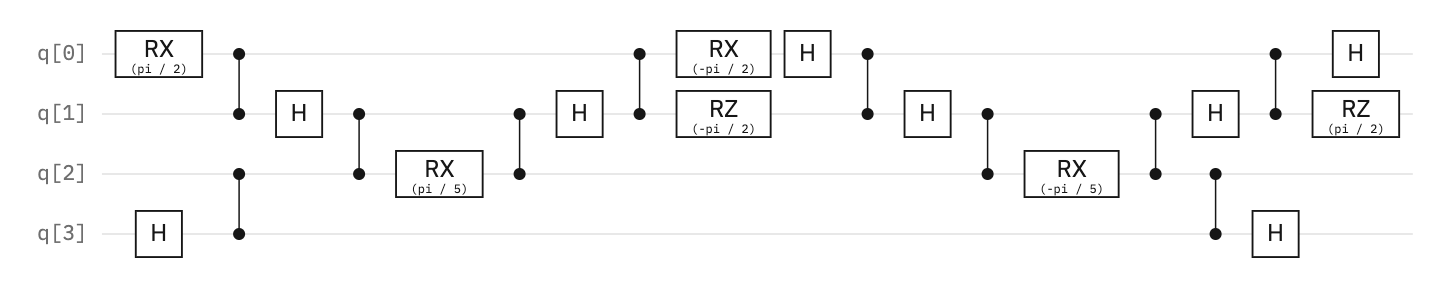
\includegraphics[width=\textwidth]{fig12_h2.png}
\end{center}

\subsection{LiH (Fig.~13): 18 CZ, 19 single-qubit gates}
Strings (from the three doubles; one string each):
\begin{equation}
P_1=Y_0X_1X_3Z_4X_5,\qquad
P_3=Y_0Z_1X_2X_3Z_4X_5,\qquad
P_2=Y_0Z_1X_2X_3X_4 .
\end{equation}
The figure applies them in the order $P_1,P_3,P_2$ (the paper's Eq.~(23)
writes $P_1,P_2,P_3$; $P_1$ and $P_3$ anticommute, so the order is part of
the ansatz definition --- both are legitimate one-parameter-per-term
ans\"atze). The pivot is \emph{always} $q_1$, and $q_4$ acts as the hub of
the $\beta$-row subtree $\{3,4,5\}$. Verified gate list:
\begin{center}\small
\begin{tabular}{ll}
\toprule
Segment & Gates (time order)\\
\midrule
$D_1$ &
 $\RX(\tfrac{\pi}{2})_0,\,H_2,H_3,H_4,H_5$;\;
 $\mathrm{CZ}_{01},\mathrm{CZ}_{34}$;\; $\mathrm{CZ}_{45}$;\; $H_4$;\; $\mathrm{CZ}_{14}$\\
rot.\ 1 & $\RX(\tfrac{\pi}{5})_1 \Rightarrow P_1=Y_0X_1X_3Z_4X_5$\\
$C_1$ & $\mathrm{CZ}_{14}$;\; $\mathrm{CZ}_{01}$;\; $H_1$;\;
        $\mathrm{CZ}_{01}$;\; $\mathrm{CZ}_{12}$;\; $\mathrm{CZ}_{14}$\\
rot.\ 2 & $\RX(\tfrac{\pi}{5})_1 \Rightarrow P_3=Y_0Z_1X_2X_3Z_4X_5$\\
$C_2$ & $\mathrm{CZ}_{14}$;\; $H_4$;\; $\mathrm{CZ}_{45}$;\;
        $\mathrm{CZ}_{34},H_5$;\; $H_4$;\; $\mathrm{CZ}_{34}$;\; $H_4$;\; $\mathrm{CZ}_{14}$\\
rot.\ 3 & $\RX(\tfrac{\pi}{5})_1 \Rightarrow P_2=Y_0Z_1X_2X_3X_4$\\
$D_3^\dagger$ & $\mathrm{CZ}_{14}$;\; $\mathrm{CZ}_{12},H_4$;\; $H_2$;\;
        $\mathrm{CZ}_{01},\mathrm{CZ}_{34}$;\; $\RX(-\tfrac{\pi}{2})_0,\,H_1,\,H_3$\\
\bottomrule
\end{tabular}
\end{center}
Things to notice (the user's two hints in action):
\begin{itemize}
\item \textbf{Shared factors stay put.} $P_1\!\to\!P_3$ share
  $Y_0$ and the whole $\{3,4,5\}$ subtree ($X_3Z_4X_5$): $C_1$ contains only
  6 gates --- it re-attaches $q_4$, flips the pivot letter
  $X_1\!\to\!Z_1$ (the $\mathrm{CZ}_{01}\,H_1\,\mathrm{CZ}_{01}$ sandwich,
  keeping $Y_0$ hooked), and hangs the new $X_2$ via $\mathrm{CZ}_{12}$
  ($H_2$ was pre-placed in the very first layer!). $P_3\!\to\!P_2$ share
  $Y_0Z_1X_2X_3$: $C_2$ only rebuilds the $\{3,4,5\}$ subtree
  ($Z_4X_5 \to X_4$, dropping $q_5$).
\item \textbf{Order matters.} The chosen order $P_1,P_3,P_2$ maximises the
  overlap of \emph{consecutive} strings (e.g.\ $P_3,P_2$ share a weight-4
  prefix). A bad order (e.g.\ $P_3$ between two strings it overlaps less)
  costs extra CZs. Without any sharing, the three rotations would need
  $2(5\!-\!1)+2(6\!-\!1)+2(5\!-\!1)=26$ CZs; sharing brings it to 18.
\end{itemize}
\begin{center}
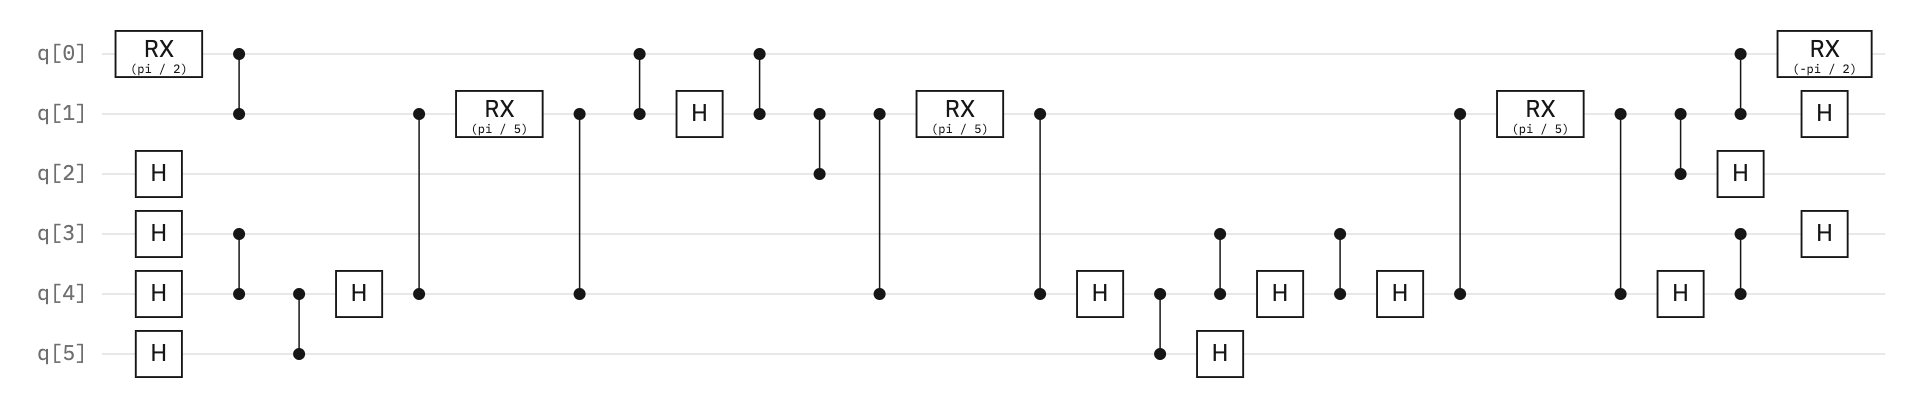
\includegraphics[width=\textwidth]{fig13_lih.png}
\end{center}

\subsection{F$_2$ (Fig.~14): 50 CZ, 63 single-qubit gates}
All five doubles share $\ad{11}\ad{5}$, so all five strings end in
$\dots X_5\,\dots X_{11}$ and are nested:
\begin{equation}
\begin{aligned}
S_1&=Y_0Z_1Z_2Z_3Z_4X_5\;X_6Z_7Z_8Z_9Z_{10}X_{11}\quad(\text{applied first})\\
S_2&=\phantom{Y_0}Y_1Z_2Z_3Z_4X_5\;\phantom{X_6}X_7Z_8Z_9Z_{10}X_{11}\\
&\;\;\vdots\\
S_5&=\phantom{Y_0Z_1Z_2Z_3}X_4X_5\;\phantom{X_6Z_7Z_8Z_9}Y_{10}X_{11}.
\end{aligned}
\end{equation}
The first block (verified to implement $e^{-i\frac{\pi}{10}S_1}$) shows the
hardware-aware ladder at its best --- everything is nearest-neighbour on the
$2\times 6$ grid and maximally parallel:
\begin{center}\small
\begin{tabular}{ll}
\toprule
Layer & Gates\\
\midrule
basis & $\RX(\tfrac{\pi}{2})_0$, $H_{1\dots 11}$\\
CZ (parallel) & $\mathrm{CZ}_{01},\ \mathrm{CZ}_{45},\ \mathrm{CZ}_{67},\ \mathrm{CZ}_{10,11}$\\
$H$ & $H_1, H_4, H_7, H_{10}$\\
CZ (parallel) & $\mathrm{CZ}_{12},\ \mathrm{CZ}_{34},\ \mathrm{CZ}_{78},\ \mathrm{CZ}_{9,10}$\\
$H$ & $H_2, H_8$\\
CZ & $\mathrm{CZ}_{23},\ \mathrm{CZ}_{89}$\\
$H$ & $H_9$\\
CZ & $\mathrm{CZ}_{39}$ \quad (the single vertical link between the rows)\\
rotation & $\RX(\tfrac{\pi}{5})_3$\\
\bottomrule
\end{tabular}
\end{center}
Each row fans its parity into a hub ($q_3$ top, $q_9$ bottom) as a balanced
tree of depth 3 (vs.\ depth 11 for a staircase). After the rotation, the
circuit does \emph{not} uncompute everything: each subsequent block peels
one rung off each row ($q_0,q_6$ drop out after $S_1$; $q_1,q_7$ after
$S_2$, \dots), migrates the $Y$-end one qubit to the right
(the $\RX(\mp\pi/2)$/$H$ pairs visible mid-circuit in Fig.~14), and relinks
the hubs one step over ($\mathrm{CZ}_{39}\to\mathrm{CZ}_{28}\to
\mathrm{CZ}_{17}\dots$), reusing the still-standing $X_5/X_{11}$ ends.
Summing it up gives the published 50 CZ + 63 single-qubit gates, against
$22+18+14+10+6=70$ CZs without sharing and $2920$ for textbook UCCSD.
\begin{center}
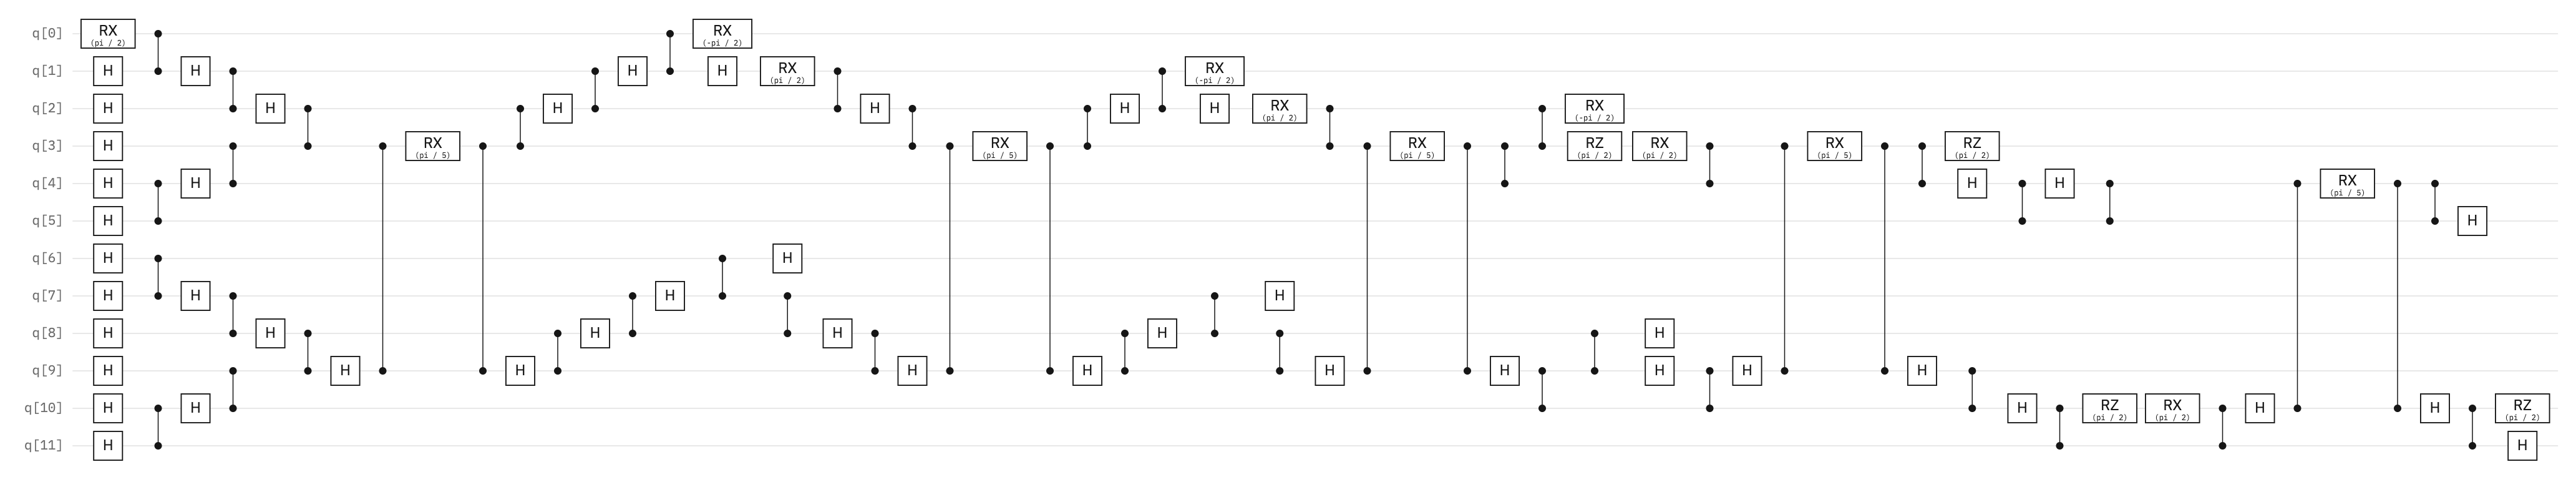
\includegraphics[width=\textwidth]{fig14_f2.png}
\end{center}

% =====================================================================
\section{The recipe in five lines}
% =====================================================================
\begin{enumerate}
\item \textbf{Select} doubles by point-group symmetry + classically computed
  energy gain (ADAPT-style screening, classically efficient on a
  determinant reference).
\item \textbf{JW-map} each double; \textbf{keep one odd-$Y$ Pauli string}
  per double (it generates the same Givens rotation on the reference;
  rescaled angle absorbed by VQE). $\Rightarrow$ $8\times$ fewer
  exponentials.
\item \textbf{Order} the strings so consecutive ones share maximal tensor
  factors (guaranteed by shared $\ad{}/\an{}$ indices, e.g.\
  $\ad{11}\ad{5}$ in every F$_2$ double).
\item \textbf{Compile} each $e^{-i\frac{\alpha}{2}P}$ as
  $D^\dagger \RX(\alpha)_p D$ with $D$ a CZ/H/$\RX(\pm\frac{\pi}{2})$
  parity \emph{tree} matched to the chip: rows fan in parallel into two
  vertically adjacent hubs, one vertical CZ joins them.
\item \textbf{Cancel} at every interface: emit only
  $C_k = D_{k+1}D_k^\dagger$, leaving shared ladder segments in place.
  Sanity check: total Clifford product $=\mathbb{1}$ and each frame
  $D_k^\dagger X_{p_k} D_k$ equals the intended string (this is exactly what
  the companion Python script automates).
\end{enumerate}

\paragraph{Verification summary (from \texttt{build\_uccsd\_circuits.py}).}
H$_2$: transcribed Fig.~12 $=$ Eq.~(22) with $\theta=\pi/10$, global phase
$1$; 10 CZ + 14 1q. LiH: transcribed Fig.~13 $=$
$e^{-i\frac{\pi}{10}P_2}e^{-i\frac{\pi}{10}P_3}e^{-i\frac{\pi}{10}P_1}$,
global phase $1$; 18 CZ + 19 1q. F$_2$: first block $=$ first factor of
Eq.~(24); full-circuit counts as published (50 CZ + 63 1q).

\end{document}
